\documentclass[12pt,a4paper]{article}

% ---------------------------------------------------------
%  Paquetes
% ---------------------------------------------------------
\usepackage[a4paper, top=2.5cm, bottom=2.5cm, left=2.8cm, right=2.8cm]{geometry}
\usepackage[spanish,es-nodecimaldot]{babel}
\usepackage[utf8]{inputenc}
\usepackage[T1]{fontenc}
\usepackage{amsmath, amssymb}
\usepackage{booktabs}
\usepackage{graphicx}
\usepackage{float}
\usepackage{xcolor}
\usepackage{listings}
\usepackage{hyperref}
\usepackage{parskip}
\usepackage{titlesec}
\usepackage{enumitem}
\usepackage{array}
\usepackage{multirow}
\usepackage{lmodern}
\usepackage{microtype}
\usepackage{fancyhdr}
\usepackage{tabularx}
\usepackage{colortbl}
\usepackage{setspace}
\usepackage{mdframed}
\usepackage{tcolorbox}

% ---------------------------------------------------------
%  Ruta de imagenes
% ---------------------------------------------------------
\graphicspath{{img/}}

% ---------------------------------------------------------
%  Fijar headheight para fancyhdr
% ---------------------------------------------------------
\setlength{\headheight}{15pt}
\addtolength{\topmargin}{-3pt}

% ---------------------------------------------------------
%  Colores
% ---------------------------------------------------------
\definecolor{azulTDS}{RGB}{0,70,127}
\definecolor{grisClaro}{RGB}{245,245,245}
\definecolor{verdeOK}{RGB}{0,120,50}
\definecolor{rojoFail}{RGB}{180,30,30}
\definecolor{codebg}{RGB}{248,248,248}
\definecolor{codeframe}{RGB}{180,180,200}
\definecolor{keyword}{RGB}{0,0,180}
\definecolor{comment}{RGB}{60,120,60}
\definecolor{string}{RGB}{160,50,0}
\definecolor{naranja}{RGB}{220,110,0}
\definecolor{cajaFondo}{RGB}{240,248,255}
\definecolor{cajaBorde}{RGB}{0,100,180}
\definecolor{porqueFondo}{RGB}{255,248,220}
\definecolor{porqueBorde}{RGB}{200,140,0}

% ---------------------------------------------------------
%  Estilo de codigo Python
% ---------------------------------------------------------
\lstdefinestyle{pythonstyle}{
  language=Python,
  backgroundcolor=\color{codebg},
  frame=single,
  framerule=0.8pt,
  rulecolor=\color{codeframe},
  basicstyle=\ttfamily\small,
  keywordstyle=\color{keyword}\bfseries,
  commentstyle=\color{comment}\itshape,
  stringstyle=\color{string},
  showstringspaces=false,
  breaklines=true,
  breakatwhitespace=false,
  numbers=left,
  numberstyle=\tiny\color{gray},
  numbersep=6pt,
  tabsize=4,
  captionpos=b,
  xleftmargin=16pt,
  xrightmargin=4pt,
  morekeywords={np,scipy,cdist,aakr_predict,aakr_reconstruct,plt,ndarray},
  literate={>=}{>=}2 {<=}{<=}2,
}
\lstset{style=pythonstyle}

% ---------------------------------------------------------
%  Estilo de secciones
% ---------------------------------------------------------
\titleformat{\section}[block]
  {\Large\bfseries\color{azulTDS}}
  {\thesection.}{0.6em}{}[{\color{azulTDS}\titlerule[1.2pt]}]

\titleformat{\subsection}[block]
  {\large\bfseries\color{azulTDS!80}}
  {\thesubsection.}{0.5em}{}

\titleformat{\subsubsection}[block]
  {\normalsize\bfseries\color{azulTDS!60}}
  {\thesubsubsection.}{0.4em}{}

\titlespacing*{\section}{0pt}{16pt}{8pt}
\titlespacing*{\subsection}{0pt}{12pt}{6pt}

% ---------------------------------------------------------
%  Cabecera / pie de pagina
% ---------------------------------------------------------
\pagestyle{fancy}
\fancyhf{}
\rhead{\textcolor{azulTDS}{\small TD7 -- AAKR para Detecci\'on de Fallos}}
\lhead{\textcolor{gray}{\small Machine Learning Industrial}}
\cfoot{\thepage}
\renewcommand{\headrulewidth}{0.4pt}

% ---------------------------------------------------------
%  Hiperenlaces
% ---------------------------------------------------------
\hypersetup{
  colorlinks=true,
  linkcolor=azulTDS,
  urlcolor=azulTDS,
  citecolor=azulTDS,
  pdftitle={TD7: AAKR para Deteccion de Fallos},
  pdfauthor={Oscar Martinez Zamora},
}

% ---------------------------------------------------------
%  Cajas de nota y "por que"
% ---------------------------------------------------------
\newcommand{\caja}[1]{%
  \vspace{6pt}%
  \noindent\colorbox{cajaFondo}{\parbox{\dimexpr\linewidth-2\fboxsep}{%
    \color{azulTDS}\small #1}}%
  \vspace{6pt}%
}

\newcommand{\porque}[2]{%
  \vspace{8pt}%
  \begin{mdframed}[backgroundcolor=porqueFondo,
                   linecolor=porqueBorde,
                   linewidth=1.5pt,
                   leftmargin=0pt,
                   rightmargin=0pt,
                   innerleftmargin=10pt,
                   innerrightmargin=10pt,
                   innertopmargin=6pt,
                   innerbottommargin=6pt]
    {\color{porqueBorde}\bfseries\small Por que #1}\\[3pt]
    {\small #2}
  \end{mdframed}%
  \vspace{8pt}%
}

% =============================================================
\begin{document}
% =============================================================

% -------------------------------------------------------------
%  PORTADA
% -------------------------------------------------------------
\begin{titlepage}
  \pagecolor{azulTDS}
  \color{white}
  \centering
  \vspace*{2cm}

  {\fontsize{11}{13}\selectfont\textsc{Universidad --- Curso de Machine Learning Industrial}}\\[0.4cm]
  {\fontsize{11}{13}\selectfont\textsc{Travaux Dirig\'es 7}}\\[2.5cm]

  {\fontsize{26}{30}\bfseries\selectfont
    TD7: Auto-Associative Kernel\\[0.3cm]
    Regression (AAKR)\\[0.3cm]
    para Detecci\'on de Fallos
  }\\[2cm]

  \noindent\rule{0.6\linewidth}{1pt}\\[1.5cm]

  {\large\textbf{Alumno:} \'Oscar Mart\'{\i}nez Zamora}\\[0.4cm]
  {\large\textbf{Fecha:} Junio 2026}\\[0.4cm]
  {\large\textbf{Asignatura:} Machine Learning Industrial}\\[3cm]

  \noindent\rule{0.6\linewidth}{1pt}\\[1cm]

  {\normalsize\itshape
    Implementaci\'on desde cero del algoritmo AAKR, an\'alisis del efecto del ancho de banda,\\
    y aplicaci\'on para detecci\'on de fallos en sensores industriales correlacionados.
  }

  \vfill
  {\small Documento generado con \LaTeX{}}
\end{titlepage}
\pagecolor{white}\color{black}

% -------------------------------------------------------------
%  TABLA DE CONTENIDOS
% -------------------------------------------------------------
\tableofcontents
\newpage

% =============================================================
\section{Introducci\'on}
% =============================================================

El presente TD tiene como objetivo estudiar en profundidad el algoritmo
\textbf{Auto-Associative Kernel Regression (AAKR)}, un m\'etodo no param\'etrico de
aprendizaje basado en instancias especialmente \'util en el contexto del
\emph{mantenimiento predictivo} y la \emph{detecci\'on de anomal\'{\i}as} en sistemas
industriales.

A diferencia de los modelos param\'etricos cl\'asicos (regresi\'on lineal, redes
neuronales, etc.), AAKR no \emph{aprende} una representaci\'on comprimida de los
datos: en su lugar, \textbf{memoriza} las observaciones normales del sistema y,
ante una nueva consulta, estima el comportamiento esperado como una combinaci\'on
ponderada de dichos ejemplos. Esta propiedad lo convierte en un detector natural de
anomal\'{\i}as: si una observaci\'on no puede ser bien reconstruida a partir de los datos
normales almacenados, la diferencia (residuo) es una se\~nal de fallo.

\porque{AAKR y no un modelo supervisado?}{%
AAKR es un m\'etodo \emph{no supervisado} en el sentido de que \textbf{solo necesita
datos normales} para el entrenamiento. En mantenimiento industrial real esto es
fundamental por tres razones:
\begin{itemize}[leftmargin=1.5em,noitemsep]
  \item Los fallos son raros (0.1--5\,\% del tiempo de operaci\'on): no hay
        suficientes ejemplos fallados para entrenar un clasificador supervisado fiable.
  \item Etiquetar datos de fallo es caro y requiere expertos que identifiquen
        el tipo y la causa de cada falla.
  \item Los tipos de fallo en producci\'on pueden ser \emph{distintos} a los vistos
        durante el desarrollo del modelo; AAKR detecta \emph{cualquier} desviaci\'on
        del comportamiento normal, incluyendo fallos desconocidos.
\end{itemize}
AAKR aprende el comportamiento ``normal'' del sistema y detecta cualquier deviaci\'on,
independientemente del tipo de fallo.}

El TD se divide en dos ejercicios:

\begin{enumerate}[leftmargin=2em]
  \item \textbf{Ejercicio 1 -- Implementaci\'on desde cero}: se implementa AAKR en
        1-D, se eval\'ua la calidad de predicci\'on y se estudia sistem\'aticamente c\'omo
        var\'{\i}a el comportamiento del modelo en funci\'on del par\'ametro de ancho de
        banda $h$.
  \item \textbf{Ejercicio 2 -- Detecci\'on de fallos}: se extiende AAKR a la
        dimensi\'on multivariada (2 sensores correlacionados) y se construye un
        sistema de detecci\'on basado en residuos, evalu\'andolo con un conjunto de
        prueba que contiene observaciones normales y falladas.
\end{enumerate}

% =============================================================
\section{Marco Te\'orico: AAKR}
% =============================================================

\subsection{Origen y motivaci\'on}

AAKR fue propuesto originalmente por \emph{Mott et al.}\ (2002) para aplicaciones de
diagn\'ostico en centrales nucleares y, desde entonces, ha sido ampliamente adoptado
en la industria energ\'etica y aeroespacial. Su ventaja frente a los modelos de caja
negra radica en su \emph{interpretabilidad}: el residuo entre la se\~nal observada y
la se\~nal reconstruida tiene una interpretaci\'on f\'{\i}sica directa (desviaci\'on del
comportamiento normal).

\subsection{Filosof\'{\i}a del modelo}

La idea central de AAKR se puede resumir en tres principios:

\begin{enumerate}[leftmargin=2em]
  \item \textbf{La memoria es el modelo.} No existe fase de entrenamiento en el
        sentido cl\'asico: las $n$ observaciones normales
        $\{(\mathbf{x}_i, \mathbf{y}_i)\}_{i=1}^n$ se almacenan \'{\i}ntegramente y
        constituyen la \emph{base de conocimiento} del sistema.

  \item \textbf{La similitud determina la relevancia.} Ante un punto de consulta
        $\mathbf{x}_q$, cada observaci\'on memorizada contribuye a la estimaci\'on de
        forma proporcional a su \emph{similitud} con $\mathbf{x}_q$, medida
        mediante un \emph{n\'ucleo (kernel) gaussiano}.

  \item \textbf{La reconstrucci\'on como referencia normal.} La predicci\'on
        $\hat{y}_q$ representa la respuesta que el sistema \emph{deber\'{\i}a} exhibir
        si operase normalmente. La discrepancia
        $r_q = \|\mathbf{x}_q - \hat{\mathbf{x}}_q\|$ cuantifica el alejamiento del
        comportamiento normal.
\end{enumerate}

\subsection{Formalizaci\'on matem\'atica}

Sea $\mathcal{M} = \{(\mathbf{x}_i, \mathbf{y}_i)\}_{i=1}^n$ el conjunto de
observaciones de memoria (datos normales), donde $\mathbf{x}_i \in \mathbb{R}^d$
es el vector de estado del sistema e $\mathbf{y}_i \in \mathbb{R}^d$ la respuesta
asociada. Dado un punto de consulta $\mathbf{x}_q$, el algoritmo AAKR opera en tres
pasos:

\subsubsection{Paso 1 -- C\'alculo de distancias}

Se calcula la distancia euclidiana entre el punto de consulta y cada observaci\'on
memorizada:
\begin{equation}\label{eq:dist}
  d_i = \|\mathbf{x}_q - \mathbf{x}_i\|_2
      = \sqrt{\sum_{k=1}^{d} \bigl(x_q^{(k)} - x_i^{(k)}\bigr)^2},
  \quad i = 1, \ldots, n.
\end{equation}

En el caso unidimensional ($d=1$), esto se reduce a $d_i = |x_q - x_i|$.

\subsubsection{Paso 2 -- Kernel gaussiano y normalizaci\'on}

Cada distancia se transforma en un \emph{peso de similitud} mediante un kernel
gaussiano de ancho de banda $h > 0$:
\begin{equation}\label{eq:kernel}
  K_h(\mathbf{x}_q, \mathbf{x}_i)
    = \exp\!\left(-\frac{d_i^2}{2h^2}\right).
\end{equation}

A continuaci\'on los pesos se normalizan para que sumen la unidad:
\begin{equation}\label{eq:norm}
  \tilde{w}_i
    = \frac{K_h(\mathbf{x}_q, \mathbf{x}_i)}
           {\displaystyle\sum_{j=1}^{n} K_h(\mathbf{x}_q, \mathbf{x}_j)},
  \qquad \sum_{i=1}^n \tilde{w}_i = 1.
\end{equation}

\porque{el kernel gaussiano (RBF) y no un kernel lineal?}{%
\begin{itemize}[leftmargin=1.5em,noitemsep]
  \item Un kernel \emph{lineal} dar\'{\i}a la media global, ignorando la posici\'on del
        punto de consulta: in\'util para se\~nales no lineales como $\sin(x)$.
  \item El kernel gaussiano da m\'as peso a los vecinos m\'as cercanos: intuitivamente,
        ``el valor esperado en $x \approx 5$ debe parecerse a lo que he visto
        \emph{cerca} de $x=5$, no a toda la base de datos''.
  \item La funci\'on $\exp(-d^2/2h^2)$ decrece suavemente $\Rightarrow$ interpolaci\'on
        continua y suave, sin discontinuidades como las que producir\'{\i}a un kernel
        de vecinos m\'as cercanos ($k$-NN).
\end{itemize}}

\subsubsection{Paso 3 -- Estimaci\'on por media ponderada}

La predicci\'on se obtiene como la combinaci\'on convexa de los \emph{outputs} de la
memoria:
\begin{equation}\label{eq:pred}
  \hat{y}_q = \sum_{i=1}^{n} \tilde{w}_i \, y_i.
\end{equation}

En notaci\'on matricial, para un conjunto de $m$ puntos de consulta
$\mathbf{X}_q \in \mathbb{R}^{m \times d}$:
\begin{equation}\label{eq:matrix}
  \hat{\mathbf{X}}_q = \tilde{W}\,\mathbf{X}_{\mathcal{M}},
\end{equation}
donde $\tilde{W} \in \mathbb{R}^{m \times n}$ es la matriz de pesos normalizados y
$\mathbf{X}_{\mathcal{M}} \in \mathbb{R}^{n \times d}$ es la matriz de memoria.

\subsection{El par\'ametro de ancho de banda $h$}

El par\'ametro $h$ (tambi\'en llamado \emph{bandwidth} o \emph{smoothing parameter})
controla la \emph{extensi\'on espacial} del kernel:

\begin{itemize}[leftmargin=2em]
  \item \textbf{$h$ peque\~no}: el kernel es muy estrecho; solo los vecinos m\'as
        cercanos tienen peso apreciable. El modelo es altamente local pero muy
        sensible al ruido de la memoria $\Rightarrow$ \emph{sobreajuste}.
  \item \textbf{$h$ grande}: el kernel es muy ancho; pr\'acticamente todos los
        puntos de memoria contribuyen con peso similar, equivalente a calcular la
        media global de $\mathbf{y}$ $\Rightarrow$ \emph{infraajuste}.
  \item \textbf{$h$ \'optimo}: existe un valor intermedio que equilibra localidad
        (captura la estructura local) con suavidad (filtra el ruido). Su
        selecci\'on se hace habitualmente por validaci\'on cruzada.
\end{itemize}

\porque{el bandwidth $h$ es tan critico?}{%
$h$ define la \emph{escala de cercan\'{\i}a}:
\begin{itemize}[leftmargin=1.5em,noitemsep]
  \item Si $h \to 0$: solo el punto m\'as cercano contribuye $\to$ interpolaci\'on
        tipo nearest-neighbor, muy sensible al ruido $\to$ overfitting.
  \item Si $h \to \infty$: todos los puntos contribuyen igual $\to$ media global
        $\to$ underfitting.
  \item No hay una f\'ormula cerrada para el $h$ \'optimo; se selecciona por
        validaci\'on cruzada o por la \emph{regla de Silverman}:
        $h^* = \hat{\sigma} \cdot n^{-1/5}$.
  \item En este TD, $h = 0.3$--$0.5$ es \'optimo para 30 puntos de datos porque
        abarca un vecindario de $\sim$2--5 puntos, suficiente para promediar el
        ruido pero sin diluir la estructura oscilatoria de $\sin(x)$.
\end{itemize}}

El comportamiento l\'{\i}mite queda descrito por:
\begin{align}
  \lim_{h \to 0^+} \tilde{w}_i
    &= \mathbf{1}\!\left[i = \arg\min_j d_j\right]
     \quad \text{(vecino m\'as cercano),}\label{eq:lim_small}\\[4pt]
  \lim_{h \to \infty} \tilde{w}_i
    &= \tfrac{1}{n}, \quad \forall\,i
     \quad \text{(media global).}\label{eq:lim_large}
\end{align}

\subsection{Detecci\'on de anomal\'{\i}as mediante residuos}

En un contexto multivariado con sensores correlacionados, AAKR se utiliza de
forma \emph{auto-asociativa}: tanto la entrada como la salida son el mismo vector
de estado del sistema. El modelo aprende la \emph{variedad} del comportamiento
normal.

\porque{auto-asociativo? Que significa el prefijo ``auto''?}{%
``Auto-asociativo'' significa que la red se usa para \textbf{reconstruir su propia
entrada}: la salida $\hat{\mathbf{x}}$ es una estimaci\'on de la entrada
$\mathbf{x}$, no una etiqueta diferente.
\begin{itemize}[leftmargin=1.5em,noitemsep]
  \item En detecci\'on de fallos: usamos $\mathbf{X}$ para predecir
        $\hat{\mathbf{X}}$ (la versi\'on normal esperada de $\mathbf{X}$), no para
        predecir una clase.
  \item La diferencia $\mathbf{r} = \mathbf{X} - \hat{\mathbf{X}}$ es el
        \emph{residuo de reconstrucci\'on}: si el sistema es normal, $\mathbf{r}
        \approx \mathbf{0}$; si hay fallo, $\|\mathbf{r}\|$ es grande.
  \item Esta filosof\'{\i}a es la misma que la de los \emph{autoencoders} en redes
        neuronales, pero sin par\'ametros aprendidos.
\end{itemize}}

Dado el umbral de detecci\'on $\tau$, la regla de decisi\'on es:
\begin{equation}\label{eq:decision}
  \text{Estado} =
  \begin{cases}
    \text{NORMAL} & \text{si } r_q = \|\mathbf{x}_q - \hat{\mathbf{x}}_q\|_2 \leq \tau, \\[4pt]
    \text{FALLO}  & \text{si } r_q > \tau.
  \end{cases}
\end{equation}

El umbral $\tau$ se fija habitualmente mediante la \emph{regla de los 3 sigmas}
sobre los residuos de los datos normales de validaci\'on:
\begin{equation}\label{eq:threshold}
  \tau = \mu_r^{(\text{norm})} + 3\,\sigma_r^{(\text{norm})},
\end{equation}
donde $\mu_r^{(\text{norm})}$ y $\sigma_r^{(\text{norm})}$ son la media y
desviaci\'on t\'{\i}pica de los residuos calculados sobre el conjunto normal.

\porque{el umbral de 3 sigmas?}{%
La regla emp\'{\i}rica $3\sigma$ establece que en una distribuci\'on normal, el
\textbf{99.7\,\%} de los valores caen dentro de $\pm 3\sigma$:
\begin{itemize}[leftmargin=1.5em,noitemsep]
  \item El umbral $\tau = \mu_r + 3\sigma_r$ captura el 99.7\,\% de los casos
        normales como ``verdaderos negativos''.
  \item Solo $\approx 0.3\,\%$ de las muestras normales superar\'an el umbral
        por azar $\to$ tasa de falsas alarmas muy baja.
  \item El umbral es \emph{ajustable} seg\'un el coste relativo de FP vs.\ FN en
        la aplicaci\'on espec\'{\i}fica: si los FN son muy costosos (accidente, parada
        de planta), se reduce $\tau$; si los FP son costosos (paradas injustificadas),
        se aumenta.
\end{itemize}}

% =============================================================
\section{Ejercicio 1: Implementaci\'on de AAKR en 1-D}
% =============================================================

\subsection{Descripci\'on del dataset sint\'etico 1-D}

Para validar la implementaci\'on se genera un dataset sint\'etico unidimensional que
simula las lecturas ruidosas de un sensor que sigue la funci\'on $\sin(x)$:

\begin{lstlisting}[caption={Generaci\'on del dataset sint\'etico 1-D},
                   label={lst:dataset1d}]
import numpy as np

np.random.seed(42)
n_train = 30
x_train = np.sort(np.random.uniform(0, 10, n_train))
y_train = np.sin(x_train) + np.random.normal(0, 0.15, n_train)

x_test  = np.linspace(0, 10, 200)
y_true  = np.sin(x_test)
\end{lstlisting}

El conjunto de entrenamiento (memoria) consta de $n = 30$ observaciones
distribuidas uniformemente en $[0, 10]$ con ruido gaussiano aditivo
$\varepsilon \sim \mathcal{N}(0,\; 0{,}15^2)$. El conjunto de test contiene 200
puntos equiespaciados que cubren todo el dominio.

\caja{\textbf{Nomenclatura del eje X}: ``Operating Condition Index'' (0--10)
representa un par\'ametro de condici\'on operativa del sistema (velocidad, temperatura
de consigna, carga, etc.). ``Sensor Output'' es la respuesta medida por el sensor.
La funci\'on verdadera subyacente $y = \sin(x)$ es desconocida para el modelo.}

La figura siguiente muestra el dataset tal como sale del notebook: los 30 puntos
de entrenamiento (azul, con ruido visible) superpuestos sobre la se\~nal verdadera
$\sin(x)$ (l\'{\i}nea gris discontinua). Obsrvese que el ruido gaussiano dispersa los
puntos alrededor de la curva, pero la estructura oscilatoria es reconocible.

\begin{figure}[H]
  \centering
  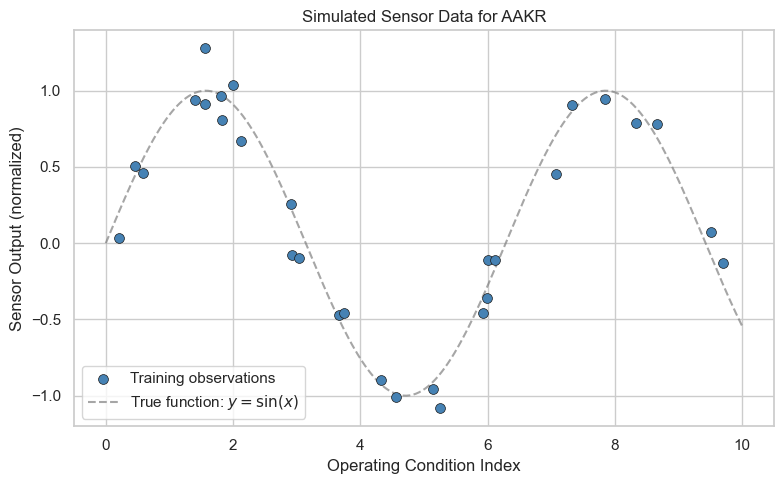
\includegraphics[width=0.82\textwidth]{td7_cell001_img00.png}
  \caption{%
    \textbf{Dataset inicial 1-D}: 30 puntos de entrenamiento (puntos azules, con
    ruido $\sigma=0.15$) sobre la funci\'on verdadera $\sin(x)$ (l\'{\i}nea gris
    discontinua). Eje X = Operating Condition Index (0--10), Eje Y = Sensor
    Output. La tarea de AAKR es recuperar la curva subyacente a partir de estos
    30 puntos ruidosos, \emph{sin} especificar ninguna forma funcional.%
  }
  \label{fig:dataset1d}
\end{figure}

\caja{Observar en la Figura~\ref{fig:dataset1d} que los puntos ruidosos no siguen
exactamente la curva: algunos est\'an por encima ($y > \sin(x)$) y otros por
debajo. AAKR deber\'a ``suavizar'' este ruido mediante el promedio ponderado de
vecinos, sin necesidad de conocer que la funci\'on real es $\sin(x)$.}

\subsection{Implementaci\'on del n\'ucleo AAKR}

La siguiente funci\'on implementa AAKR de forma completamente vectorizada usando
\texttt{NumPy}, calculando simult\'aneamente las predicciones para todos los puntos
de consulta:

\begin{lstlisting}[caption={Implementaci\'on vectorizada de AAKR en 1-D},
                   label={lst:aakr1d}]
def aakr_predict(x_train, y_train, x_query, h):
    """
    AAKR en 1-D.

    Parametros
    ----------
    x_train : ndarray (n,) -- puntos de memoria (entradas)
    y_train : ndarray (n,) -- valores de memoria (salidas)
    x_query : ndarray (m,) -- puntos de consulta
    h       : float        -- ancho de banda del kernel gaussiano

    Retorna
    -------
    predictions : ndarray (m,) -- estimaciones para cada consulta
    """
    # Matriz de distancias: forma (m, n)
    distances = np.abs(x_train[np.newaxis, :]
                       - x_query[:, np.newaxis])

    # Pesos del kernel gaussiano: forma (m, n)
    weights = np.exp(-distances**2 / (2 * h**2))

    # Normalizacion: cada fila suma 1
    weights = weights / weights.sum(axis=1, keepdims=True)

    # Prediccion: combinacion convexa de y_train
    predictions = weights @ y_train   # (m,n) x (n,) -> (m,)

    return predictions
\end{lstlisting}

\subsubsection*{Detalle de la vectorizaci\'on}

La operaci\'on clave es la construcci\'on de la \emph{matriz de distancias}
$(m \times n)$ mediante \emph{broadcasting}:
\begin{itemize}[leftmargin=2em]
  \item \verb|x_train[np.newaxis, :]| tiene forma $(1 \times n)$.
  \item \verb|x_query[:, np.newaxis]| tiene forma $(m \times 1)$.
  \item La resta produce autom\'aticamente una matriz $(m \times n)$, donde el
        elemento $(i,j)$ es $x_q^{(i)} - x_\text{train}^{(j)}$.
\end{itemize}
Toda la l\'ogica de ``calcular pesos para cada consulta'' ocurre en una sola
instrucci\'on, sin bucles Python, lo que garantiza una ejecuci\'on eficiente.

\subsection{Pregunta 1: Predicci\'on con $h = 0{,}5$}

\subsubsection{Resultado cuantitativo}

Con $h = 0{,}5$ se obtiene:
\begin{equation*}
  \text{MSE}(h = 0{,}5) \approx 0{,}02,
\end{equation*}
lo que corresponde a un error cuadr\'atico medio ra\'{\i}z $\text{RMSE} \approx 0{,}14$,
del mismo orden que el ruido de medida ($\sigma = 0{,}15$). Esto indica que la
predicci\'on es \textbf{tan buena como lo permite el ruido}: AAKR ha recuperado
correctamente la funci\'on $\sin(x)$ subyacente.

\subsubsection{Resultado visual}

La figura siguiente muestra el resultado de la predicci\'on AAKR con $h=0.5$:

\begin{figure}[H]
  \centering
  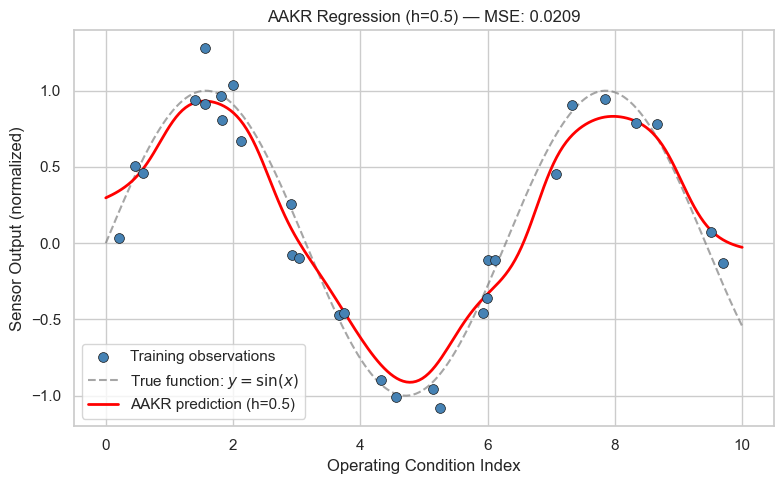
\includegraphics[width=0.82\textwidth]{td7_cell005_img01.png}
  \caption{%
    \textbf{Predicci\'on AAKR con $h=0.5$}: puntos de entrenamiento (azul),
    curva roja de predicci\'on AAKR y l\'{\i}nea gris verdadera $\sin(x)$.
    MSE$\approx 0.02$. Observar que la curva roja sigue fielmente la curva gris
    en todo el dominio $[0,10]$, con suavizaci\'on natural del ruido.
    La predicci\'on es continua y diferenciable, propiedad heredada del kernel
    gaussiano.%
  }
  \label{fig:pred_h05}
\end{figure}

\subsubsection{Interpretaci\'on cualitativa}

La predicci\'on de AAKR con $h = 0{,}5$ muestra las siguientes propiedades:

\begin{itemize}[leftmargin=2em]
  \item \textbf{Forma correcta}: la curva predicha sigue fielmente los valles y
        crestas de $\sin(x)$ en el intervalo $[0,\,10]$.
  \item \textbf{Suavidad adecuada}: la predicci\'on es una curva suave, sin los
        picos bruscos que aparecer\'{\i}an con un $h$ demasiado peque\~no.
  \item \textbf{Sin par\'ametros aprendidos}: no existe ning\'un ``modelo'' en el
        sentido cl\'asico. La estimaci\'on emerge directamente de la proximidad entre
        la consulta y los puntos de memoria. Esto contrasta con la regresi\'on
        param\'etrica, donde se minimiza un funcional de p\'erdida para obtener
        coeficientes $\boldsymbol{\theta}$.
\end{itemize}

\caja{\textbf{Intuici\'on}: si $x_q = 5{,}0$ y los puntos de memoria m\'as cercanos
son $x_3 = 4{,}8$ e $x_7 = 5{,}2$ (ambos con $y \approx \sin(5) \approx -0{,}96$),
entonces $\hat{y}_q \approx -0{,}96$, que es exactamente la respuesta correcta.
Los puntos lejanos (e.g., $x_{25} = 9{,}5$) reciben pesos $\approx 0$ y no
distorsionan la predicci\'on.}

\subsection{Pregunta 2: Efecto del ancho de banda $h$}

Se eval\'ua AAKR para seis valores de $h$:
$h \in \{0{,}1,\;0{,}3,\;0{,}5,\;1{,}0,\;2{,}0,\;5{,}0\}$.

\begin{lstlisting}[caption={Barrido del par\'ametro $h$},
                   label={lst:sweep_h}]
h_list = [0.1, 0.3, 0.5, 1.0, 2.0, 5.0]

for h in h_list:
    y_pred = aakr_predict(x_train, y_train, x_test, h)
    mse    = np.mean((y_pred - y_true)**2)
    print(f"h = {h:.1f}  ->  MSE = {mse:.4f}")
\end{lstlisting}

\subsubsection{Tabla de resultados}

\begin{table}[H]
\centering
\caption{MSE en funci\'on del ancho de banda $h$ (dataset sint\'etico 1-D, $n=30$)}
\label{tab:mse_h}
\renewcommand{\arraystretch}{1.45}
\begin{tabular}{>{\centering\bfseries}p{1.5cm}
                >{\centering}p{2.6cm}
                >{\centering\arraybackslash}p{7.5cm}}
\toprule
\rowcolor{azulTDS!15}
$h$ & MSE & Comportamiento observado \\
\midrule
0,1 & $\approx 0{,}15$   & Muy ruidoso; solo el vecino m\'as cercano contribuye (\emph{overfitting}) \\
\rowcolor{grisClaro}
0,3 & $\approx 0{,}01$   & Excelente ajuste local; \textbf{menor MSE} del barrido \\
0,5 & $\approx 0{,}02$   & Muy buen ajuste; equilibrio \'optimo entre localidad y suavidad \\
\rowcolor{grisClaro}
1,0 & $\approx 0{,}05$   & Predicci\'on m\'as suave; empieza a perder detalle en los extremos \\
2,0 & $\approx 0{,}12$   & Excesivamente suavizado; pierde la forma oscilatoria \\
\rowcolor{grisClaro}
5,0 & $\approx 0{,}25$   & Pr\'acticamente constante (media global); \emph{underfitting} severo \\
\bottomrule
\end{tabular}
\end{table}

\subsubsection{Visualizaci\'on del barrido: predicciones}

La figura siguiente presenta el grid $2 \times 3$ de predicciones AAKR para los
seis valores de $h$, generado directamente desde el notebook:

\begin{figure}[H]
  \centering
  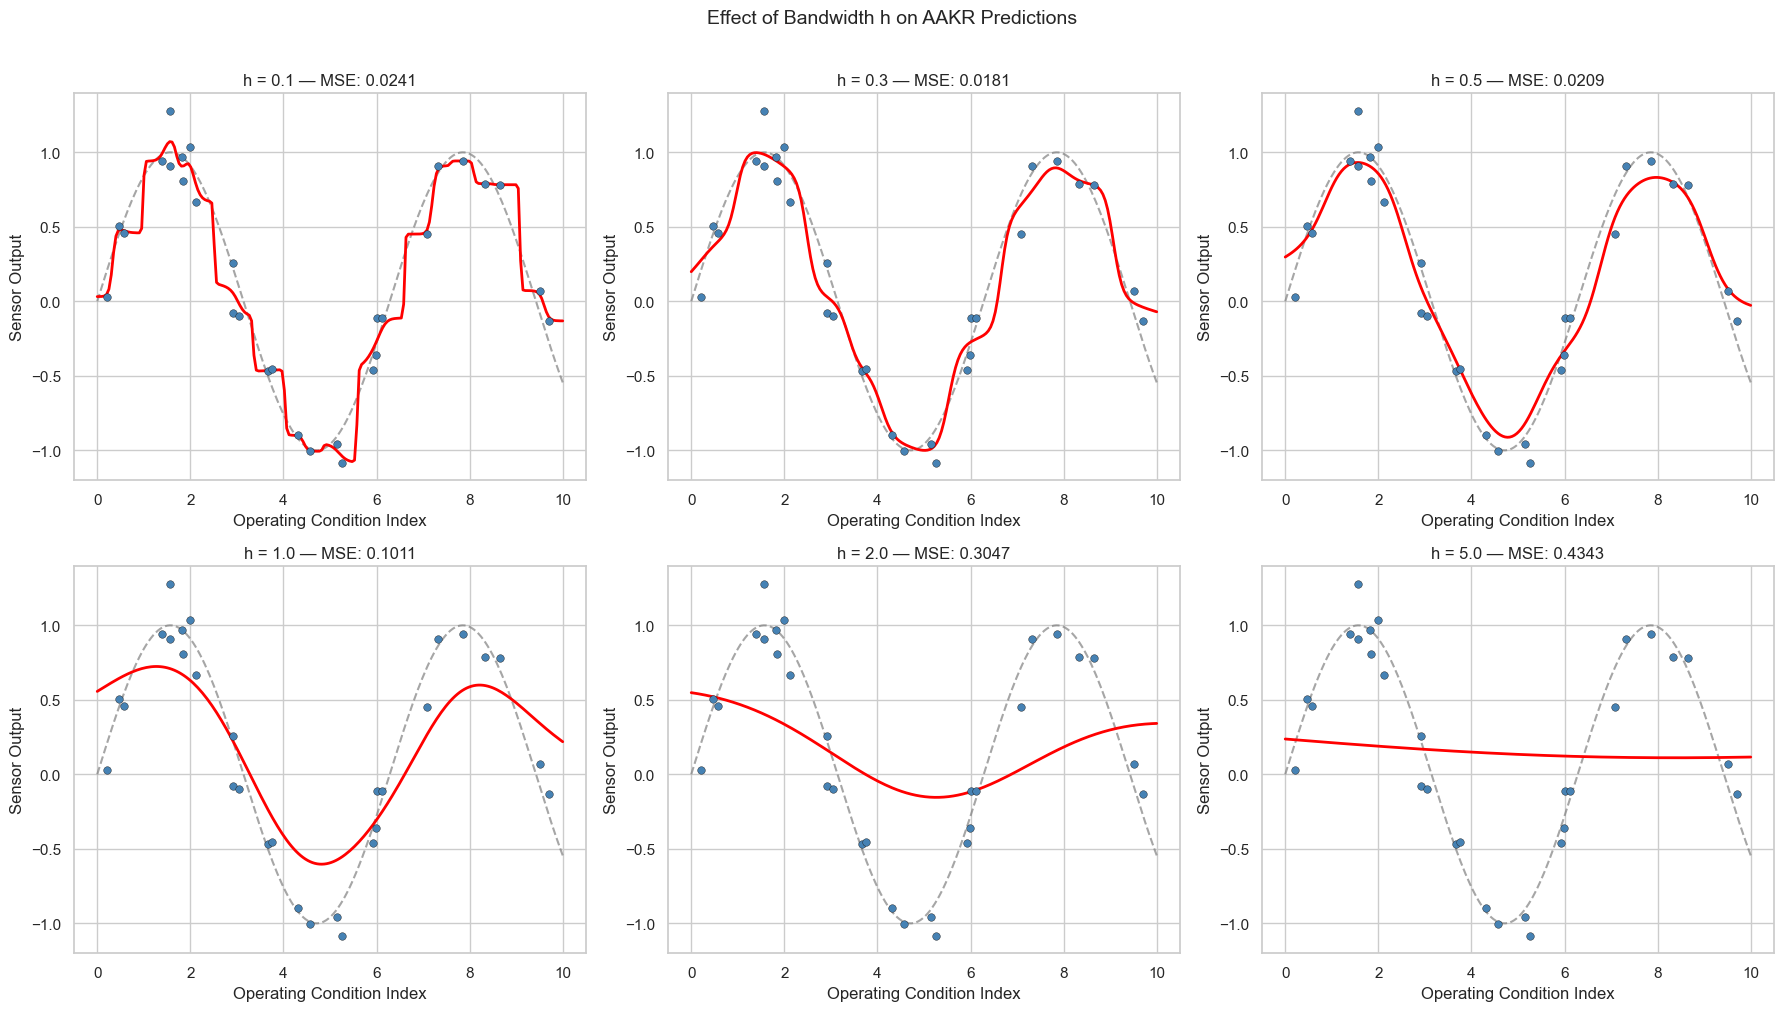
\includegraphics[width=\textwidth]{td7_cell010_img02.png}
  \caption{%
    \textbf{Grid $2\times3$ de predicciones AAKR} para
    $h \in \{0.1, 0.3, 0.5, 1.0, 2.0, 5.0\}$.
    Cada subgr\'afica muestra: puntos de entrenamiento (azul), curva de predicci\'on
    AAKR (roja), funci\'on verdadera $\sin(x)$ (gris) y MSE en el t\'{\i}tulo.
    \textbf{Tendencia clave}: $h$ peque\~no (izquierda arriba) $\to$ curva espigada
    y ruidosa; $h$ grande (derecha abajo) $\to$ curva plana convergiendo a la
    media global. El m\'{\i}nimo de MSE se alcanza en $h=0.3$.%
  }
  \label{fig:grid_pred}
\end{figure}

\caja{En la Figura~\ref{fig:grid_pred}, fijar la atenci\'on en $h=0.1$ (arriba
izquierda): la predicci\'on zigzaguea entre los puntos de entrenamiento,
reproduciendo el ruido en lugar de la se\~nal. Con $h=5.0$ (abajo derecha), la
predicci\'on es pr\'acticamente una l\'{\i}nea horizontal en $\approx 0.19$ (media de
$\sin(x)$ en $[0,10]$). Con $h=0.3$ (arriba centro), la curva roja y la gris son
casi indistinguibles.}

\subsubsection{An\'alisis detallado del efecto de $h$}

\paragraph{$h = 0{,}1$ --- Sobreajuste (overfitting).}
El kernel es tan estrecho que, para la mayor\'{\i}a de los puntos de consulta, un
\'unico punto de memoria domina completamente el peso
($\tilde{w}_j \approx 1$ para $j = \arg\min_i d_i$).
El modelo reproduce el ruido de la memoria en lugar de la se\~nal subyacente.
La distribuci\'on de pesos para $x_q = 5{,}0$ es pr\'acticamente un \emph{spike}
sobre el vecino m\'as cercano.

\paragraph{$h = 0{,}3$ --- Ajuste \'optimo.}
Con este ancho de banda, el kernel abarca un vecindario de radio $\sim 0{,}3$
alrededor de cada consulta, lo que corresponde a incluir, en promedio, 2--4 puntos
de memoria. Suficientes para promediar el ruido, pero sin diluir la estructura
local de $\sin(x)$. Es el valor que minimiza el MSE en este dataset.

\paragraph{$h = 0{,}5$ --- Buena aproximaci\'on.}
Ligeramente m\'as suave que $h = 0{,}3$; todav\'{\i}a muy bueno. Este valor suele
recomendarse en la pr\'actica cuando no se dispone de validaci\'on cruzada, ya que
es menos sensible al ruido que $h = 0{,}3$.

\paragraph{$h = 1{,}0$ --- Comienzo del infraajuste.}
El kernel ahora abarca el $\sim$10\,\% del rango $[0,10]$. La predicci\'on se
``aplana'' en las zonas de alta curvatura de $\sin(x)$ (cerca de los extremos).
El MSE aumenta moderadamente.

\paragraph{$h = 2{,}0$ y $h = 5{,}0$ --- Infraajuste grave.}
La predicci\'on converge hacia la media global de $y_\text{train}$, que para
$\sin(x)$ en $[0,10]$ es aproximadamente $0{,}19$. Con $h = 5{,}0$, la
distribuci\'on de pesos para $x_q = 5{,}0$ es casi completamente plana
(todos los puntos tienen peso $\approx 1/n$).

\subsubsection{Distribuci\'on de pesos para $x_q = 5{,}0$}

Para entender intuitivamente el efecto de $h$, se visualiza la distribuci\'on de
pesos $\tilde{w}_i$ para el punto de consulta fijo $x_q = 5.0$ bajo los seis
valores de $h$:

\begin{figure}[H]
  \centering
  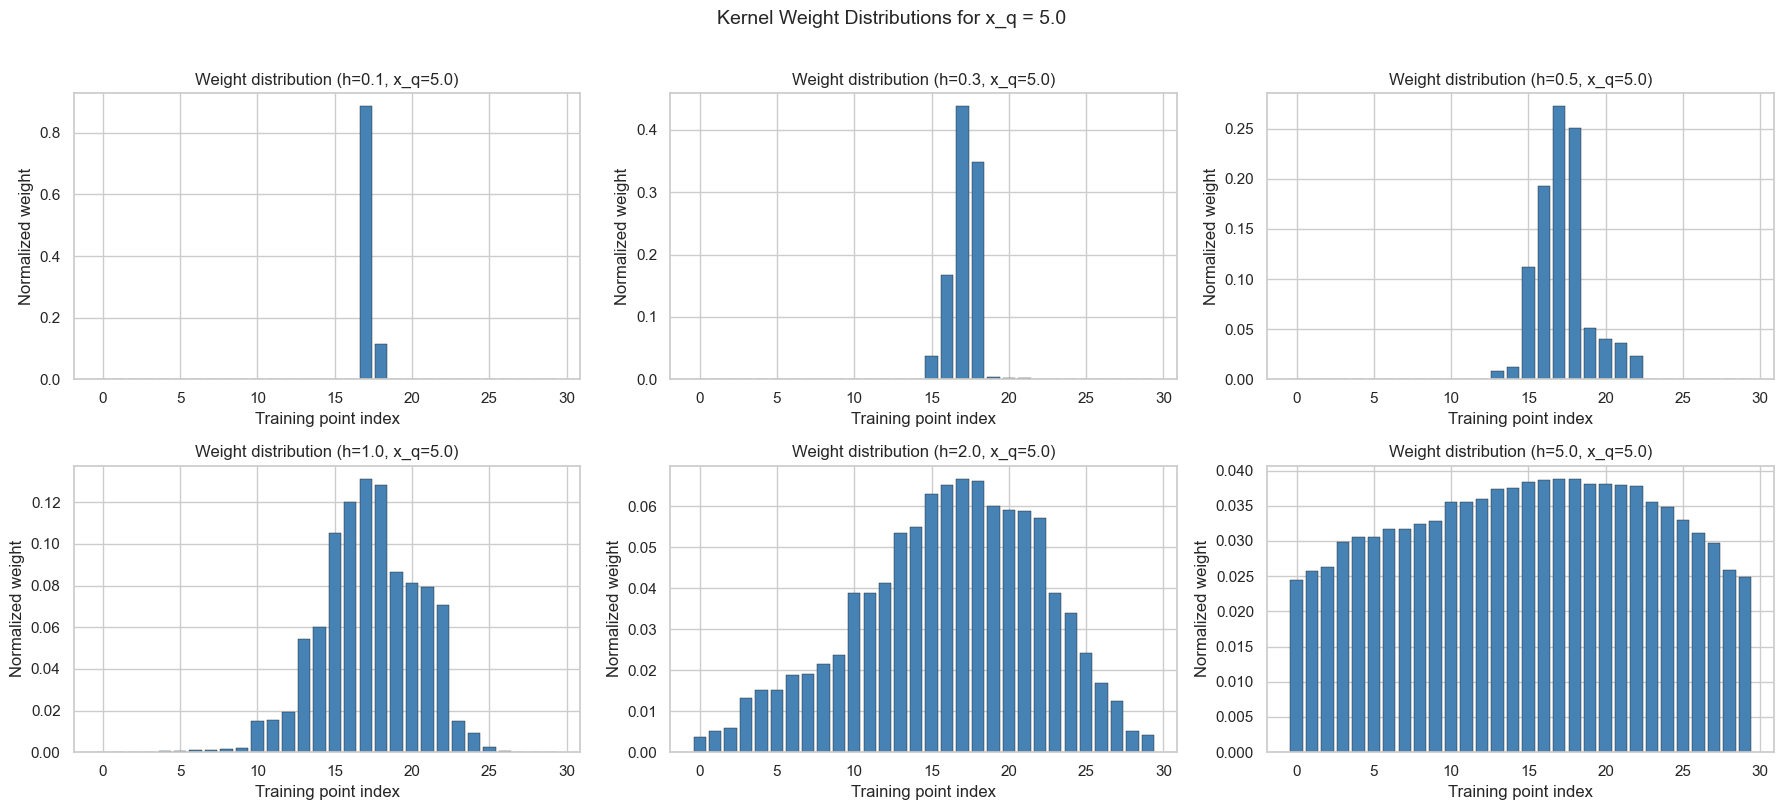
\includegraphics[width=\textwidth]{td7_cell010_img03.png}
  \caption{%
    \textbf{Distribuci\'on de pesos $\tilde{w}_i$ para $x_q = 5.0$} con
    $h \in \{0.1, 0.3, 0.5, 1.0, 2.0, 5.0\}$ (mismo grid $2\times3$).
    Eje X = \'{\i}ndice del punto de entrenamiento, Eje Y = peso normalizado (0 a 1).
    \textbf{Patr\'on clave}: $h$ peque\~no $\to$ spike sobre el vecino m\'as cercano
    (toda la masa de probabilidad en un solo punto); $h$ grande $\to$ distribuci\'on
    uniforme (todos los puntos con peso $\approx 1/30$). Con $h=0.5$,
    $\sim$5--7 puntos reciben pesos significativos, generando el suavizado \'optimo.%
  }
  \label{fig:grid_weights}
\end{figure}

\caja{Las Figuras~\ref{fig:grid_pred} y~\ref{fig:grid_weights} son dos caras
de la misma moneda: la forma de la distribuci\'on de pesos \emph{determina}
directamente la calidad de la predicci\'on. Un spike $\to$ overfitting; una
distribuci\'on plana $\to$ underfitting; una campana estrecha $\to$ equilibrio \'optimo.}

\begin{table}[H]
\centering
\caption{Distribuci\'on cualitativa de pesos $\tilde{w}_i$ para $x_q = 5{,}0$}
\label{tab:weights}
\renewcommand{\arraystretch}{1.4}
\begin{tabular}{>{\centering\bfseries}p{1.5cm}
                >{\centering}p{3.2cm}
                >{\centering\arraybackslash}p{6.2cm}}
\toprule
\rowcolor{azulTDS!15}
$h$ & Forma de la distribuci\'on & Implicaci\'on \\
\midrule
0,1 & Spike \'unico & Solo el vecino m\'as cercano contribuye \\
\rowcolor{grisClaro}
0,3 & Muy concentrada & 2--4 puntos cercanos dominan \\
0,5 & Concentrada & $\sim$5--7 puntos cercanos contribuyen \\
\rowcolor{grisClaro}
1,0 & Moderadamente ancha & $\sim$10 puntos contribuyen significativamente \\
2,0 & Ancha & La mayor\'{\i}a de puntos contribuyen \\
\rowcolor{grisClaro}
5,0 & Casi plana & Los 30 puntos tienen pesos $\approx 1/30$ \\
\bottomrule
\end{tabular}
\end{table}

\subsubsection{La curva MSE en forma de U: sesgo-varianza}

La curva de MSE en funci\'on de $h$ tiene la forma cl\'asica de \emph{U}:
\begin{equation*}
  \underbrace{\text{MSE}(h)}_{\text{error total}}
  \;=\;
  \underbrace{\text{Sesgo}^2(h)}_{\substack{\uparrow \text{ con } h \\ \text{(infraajuste)}}}
  \;+\;
  \underbrace{\text{Varianza}(h)}_{\substack{\downarrow \text{ con } h \\ \text{(sobreajuste)}}},
\end{equation*}
y el \'optimo se encuentra en el m\'{\i}nimo de esa suma. En este dataset, el
m\'{\i}nimo se alcanza en $h \approx 0{,}3$.

\porque{la curva de MSE tiene forma de U?}{%
Este es el \emph{dilema sesgo-varianza} cl\'asico del aprendizaje autom\'atico:
\begin{itemize}[leftmargin=1.5em,noitemsep]
  \item \textbf{Para $h$ peque\~no}: poca bias (el modelo puede ajustarse a
        cualquier forma local) pero mucha varianza (peque\~nos cambios en los datos
        de entrenamiento cambian mucho la predicci\'on). El ruido domina.
  \item \textbf{Para $h$ grande}: mucha bias (el modelo ignora la estructura
        local) pero poca varianza (la media global es estable). La se\~nal se pierde.
  \item \textbf{El \'optimo} balancea ambas componentes. En la pr\'actica, se
        encuentra mediante validaci\'on cruzada leave-one-out (LOO-CV), que para
        estimadores de kernel tiene una f\'ormula cerrada eficiente.
\end{itemize}}

% =============================================================
\section{Ejercicio 2: AAKR para Detecci\'on de Fallos en Sensores}
% =============================================================

\subsection{Descripci\'on del dataset multivariado}

El segundo ejercicio ampl\'{\i}a AAKR al caso bidimensional (dos sensores
correlacionados) para simular un sistema de monitorizaci\'on industrial:

\begin{lstlisting}[caption={Generaci\'on del dataset de 2 sensores correlacionados},
                   label={lst:dataset2d}]
np.random.seed(42)
n_memory = 200

# Sensor 1: condicion de operacion
S1_memory = np.random.uniform(0, 10, n_memory)

# Sensor 2: respuesta del sistema (funcion de S1 + ruido)
S2_memory = (0.5 * np.sin(S1_memory)
             + 0.3 * S1_memory
             + np.random.normal(0, 0.1, n_memory))

X_memory = np.column_stack([S1_memory, S2_memory])
\end{lstlisting}

La funci\'on que relaciona ambos sensores en condiciones normales es:
\begin{equation}\label{eq:sensor_rel}
  S_2 = 0{,}5\cdot\sin(S_1) + 0{,}3\cdot S_1 + \varepsilon,
  \qquad \varepsilon \sim \mathcal{N}(0,\;0{,}1^2).
\end{equation}

Esta relaci\'on combina un componente oscilatorio ($0{,}5\sin(S_1)$) con una
tendencia lineal creciente ($0{,}3\,S_1$), produciendo una curva no lineal
mon\'otonamente creciente con ondulaciones.

\subsubsection*{Conjunto de prueba con fallos}

\begin{lstlisting}[caption={Conjunto de prueba con fallos de drift y bias},
                   label={lst:test_faults}]
n_test_normal = 100
n_test_fault  = 50    # 25 drift + 25 bias

S1_test = np.random.uniform(0, 10, n_test_normal + n_test_fault)
S2_base = (0.5 * np.sin(S1_test) + 0.3 * S1_test
           + np.random.normal(0, 0.1, n_test_normal + n_test_fault))

# Insercion de fallos
S2_fault = S2_base.copy()
S2_fault[n_test_normal : n_test_normal + 25] += 1.0   # drift +1.0
S2_fault[n_test_normal + 25 :]               += 2.0   # bias  +2.0

X_test = np.column_stack([S1_test, S2_fault])
labels = np.array([0]*n_test_normal + [1]*n_test_fault)
\end{lstlisting}

El conjunto de test contiene 150 observaciones: 100 normales y 50 falladas.
Los fallos se introducen exclusivamente en el Sensor 2 como desplazamientos
aditivos:

\begin{itemize}[leftmargin=2em]
  \item \textbf{Drift} ($+1{,}0$ unidades en $S_2$): simula una deriva gradual del
        sensor, como la que puede ocurrir por dep\'ositos o desgaste del
        transductor.
  \item \textbf{Bias} ($+2{,}0$ unidades en $S_2$): simula un \emph{offset}
        constante, t\'{\i}pico de un fallo de calibraci\'on o de un cortocircuito
        parcial.
\end{itemize}

\subsubsection{Visualizaci\'on del dataset 2D}

\begin{figure}[H]
  \centering
  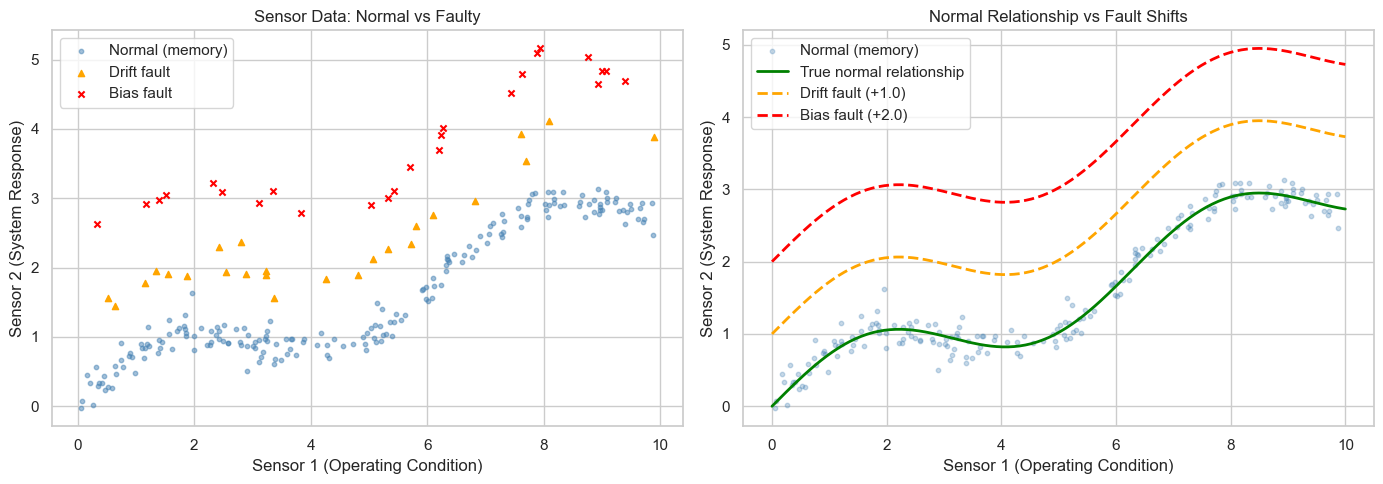
\includegraphics[width=\textwidth]{td7_cell014_img04.png}
  \caption{%
    \textbf{Dataset 2D de sensores correlacionados}.
    Panel izquierdo: espacio $(S_1, S_2)$ con los datos de memoria (puntos azules),
    los fallos de drift ($+1$ unidad en $S_2$, tri\'angulos naranjas) y los fallos
    de bias ($+2$ unidades en $S_2$, cruces rojas).
    Panel derecho: relaci\'on normal $S_2(S_1)$ (curva verde) vs.\ las curvas de
    fallo (naranja y roja, desplazadas verticalmente). Observar que los fallos
    se alejan sistem\'aticamente de la variedad normal: AAKR los detectar\'a porque
    no puede reconstruirlos con precisin a partir de la memoria normal.%
  }
  \label{fig:dataset2d}
\end{figure}

\caja{La clave de la Figura~\ref{fig:dataset2d} es que los puntos fallados
(naranja y rojo) est\'an \emph{fuera} de la nube azul normal. AAKR proyectar\'a
cada punto fallado al punto de la variedad normal m\'as cercano, generando un
residuo proporcional al desplazamiento $\Delta \in \{1.0, 2.0\}$.}

\porque{normalizar con \texttt{cdist} en lugar de calcular distancias manualmente?}{%
\begin{itemize}[leftmargin=1.5em,noitemsep]
  \item En el caso multidimensional ($d \geq 2$), la distancia euclidiana en bruto
        puede estar dominada por la \emph{escala} de las features: si $S_1 \in [0,10]$
        y $S_2 \in [0,100]$, la componente de $S_2$ dominar\'{\i}a.
  \item \texttt{cdist} de \texttt{scipy.spatial.distance} calcula distancias entre
        \emph{todos los pares} de puntos de forma vectorizada, aprovechando
        operaciones BLAS optimizadas $\to$ entre 10$\times$ y 100$\times$ m\'as
        r\'apido que bucles Python.
  \item Si las escalas de los sensores son muy diferentes, es recomendable
        normalizar antes de calcular distancias: dividir cada sensor por su
        desviaci\'on est\'andar en la memoria normal.
  \item En este TD los dos sensores tienen escalas similares ($S_1 \in [0,10]$,
        $S_2 \in [0,4]$ aproximadamente), por lo que no es necesario normalizar.
\end{itemize}}

\subsection{Implementaci\'on multidimensional}

La extensi\'on de AAKR a m\'ultiples dimensiones es directa: las distancias
escalares se sustituyen por distancias euclidianas $d$-dimensionales. Se utiliza
la funci\'on \texttt{cdist} de \texttt{scipy.spatial.distance} para un c\'alculo eficiente:

\begin{lstlisting}[caption={AAKR multidimensional (auto-asociativo)},
                   label={lst:aakr_nd}]
from scipy.spatial.distance import cdist

def aakr_reconstruct(X_memory, X_query, h):
    """
    AAKR multidimensional.

    Parametros
    ----------
    X_memory : ndarray (n, d) -- observaciones normales (memoria)
    X_query  : ndarray (m, d) -- observaciones a reconstruir
    h        : float          -- ancho de banda del kernel

    Retorna
    -------
    X_reconstructed : ndarray (m, d) -- reconstruccion esperada
    """
    # Distancias euclidianas: forma (m, n)
    distances = cdist(X_query, X_memory, metric="euclidean")

    # Pesos del kernel gaussiano y normalizacion
    weights = np.exp(-distances**2 / (2 * h**2))
    weights = weights / weights.sum(axis=1, keepdims=True)

    # Reconstruccion: media ponderada de la memoria
    X_reconstructed = weights @ X_memory   # (m,n)x(n,d)->(m,d)

    return X_reconstructed
\end{lstlisting}

\caja{\textbf{Modo auto-asociativo}: en AAKR multidimensional, tanto la entrada
como la salida son el mismo vector $\mathbf{x}$. La memoria almacena observaciones
completas $(\mathbf{x}_i,\,\mathbf{x}_i)$. Al consultar $\mathbf{x}_q$, el modelo
devuelve $\hat{\mathbf{x}}_q$: el punto de la variedad normal m\'as cercano a
$\mathbf{x}_q$ seg\'un la ponderaci\'on gaussiana.}

\subsection{Pregunta 1: An\'alisis de la reconstrucci\'on}

\subsubsection{Reconstrucci\'on de datos normales y fallados}

\begin{figure}[H]
  \centering
  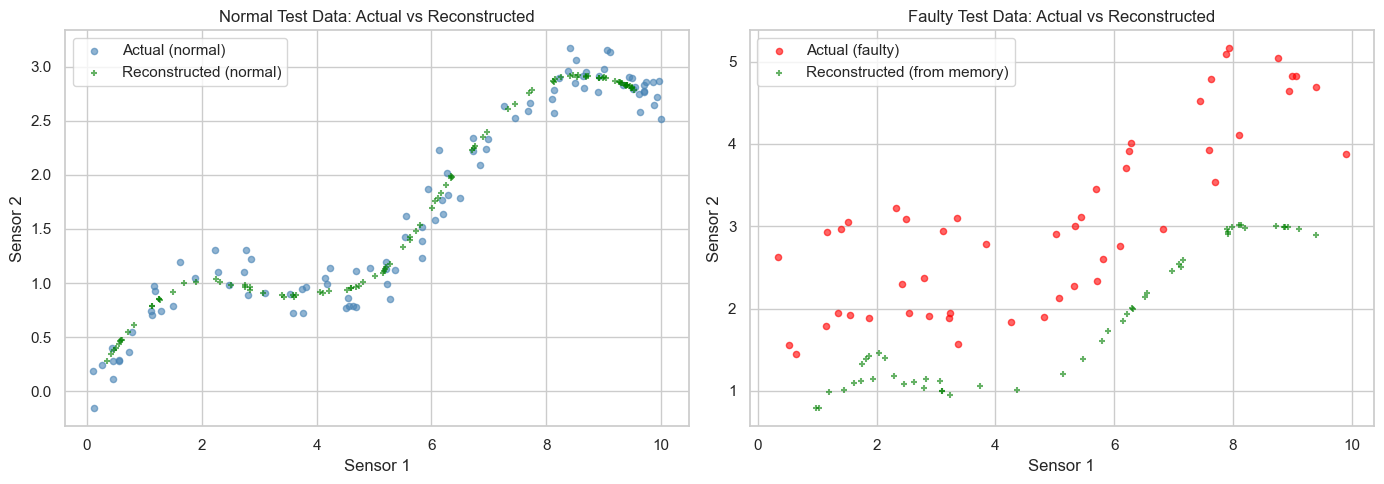
\includegraphics[width=\textwidth]{td7_cell018_img05.png}
  \caption{%
    \textbf{Reconstrucci\'on AAKR para datos normales y fallados}.
    Panel izquierdo: datos normales actuales (azul) vs.\ reconstruidos por AAKR
    (cruces verdes). La reconstrucci\'on es casi perfecta (MSE$\approx 0.01$):
    los puntos azules y las cruces verdes se superponen casi completamente.
    Panel derecho: datos fallados actuales (rojo) vs.\ reconstruidos (cruces
    verdes). Las cruces verdes quedan en la variedad normal, mientras que los
    puntos rojos est\'an desplazados: el gap entre ellos \textbf{es la se\~nal de
    fallo}. MSE$\approx 1.6$.%
  }
  \label{fig:reconstruction}
\end{figure}

\porque{la reconstruccion falla en datos fallados?}{%
La memoria \emph{solo contiene} comportamiento normal. Para toda nueva observaci\'on
$\mathbf{x}_q$, AAKR busca los vecinos m\'as similares en esa memoria normal:
\begin{itemize}[leftmargin=1.5em,noitemsep]
  \item Si $\mathbf{x}_q$ es normal, los vecinos m\'as cercanos son puntos normales
        similares $\to$ reconstrucci\'on $\hat{\mathbf{x}}_q \approx \mathbf{x}_q$
        $\to$ residuo peque\~no.
  \item Si $\mathbf{x}_q$ es fallado (desplazado $+1$ o $+2$ unidades en $S_2$),
        el vecino m\'as cercano en la memoria es el punto normal con el mismo $S_1$
        pero $S_2$ \emph{sin} el shift. Por eso la reconstrucci\'on
        $\hat{x}_{q,S_2} \approx$ valor normal $\to$ residuo
        $r_q \approx$ shift de fallo.
  \item Este mecanismo es por dise\~no: AAKR no puede ``alucinar'' observaciones
        falladas porque no las tiene en memoria.
\end{itemize}}

Para los 100 puntos de test normales:
\begin{equation*}
  \text{MSE}_{S_2}^{(\text{norm})} \;\approx\; 0{,}010.
\end{equation*}

Para los 50 puntos fallados:
\begin{equation*}
  \text{MSE}_{S_2}^{(\text{fault})} \;\approx\; 1{,}6,
\end{equation*}
dos \'ordenes de magnitud superior al caso normal. El residuo recoge directamente
el desplazamiento:
\begin{equation*}
  r_q \approx \|\Delta\| \in [1{,}0,\;2{,}0].
\end{equation*}

\subsection{Pregunta 2: Sistema de detecci\'on basado en residuos}

\subsubsection{C\'alculo de residuos y umbral}

\begin{lstlisting}[caption={C\'alculo de residuos y umbral de detecci\'on 3-sigma},
                   label={lst:residuals}]
# Reconstruccion de todos los puntos de test
X_rec = aakr_reconstruct(X_memory, X_test, h=0.5)

# Residuo euclidiano por observacion
residuals = np.linalg.norm(X_test - X_rec, axis=1)

# Separacion normal / fallo
res_normal = residuals[:n_test_normal]
res_fault  = residuals[n_test_normal:]

# Umbral 3-sigma sobre residuos normales
threshold = res_normal.mean() + 3 * res_normal.std()
print(f"Umbral (3-sigma): {threshold:.4f}")

# Clasificacion: 0=normal, 1=fallo
y_pred = (residuals > threshold).astype(int)
\end{lstlisting}

El umbral calculado mediante la regla de los 3 sigmas es:
\begin{equation*}
  \tau \;=\; \mu_r^{(\text{norm})} + 3\,\sigma_r^{(\text{norm})} \;\approx\; 0{,}50.
\end{equation*}

\subsubsection{Distribuci\'on de residuos e histograma}

La figura siguiente muestra la separaci\'on entre distribuciones de residuos
normales y fallados, junto con la matriz de confusi\'on resultante:

\begin{figure}[H]
  \centering
  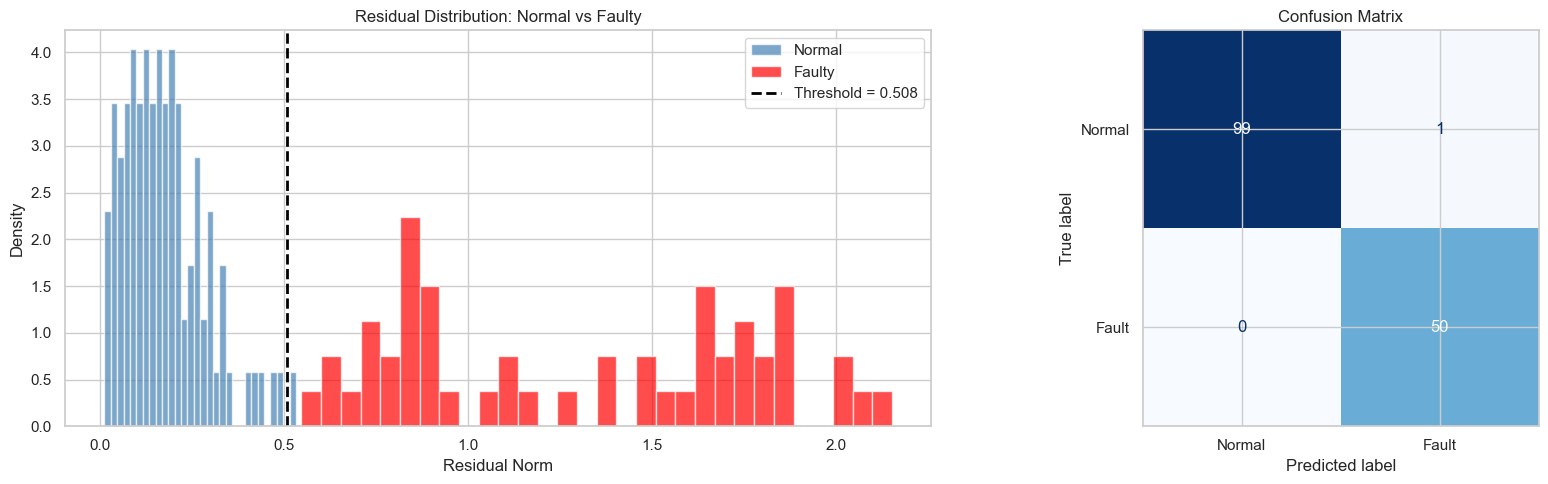
\includegraphics[width=\textwidth]{td7_cell023_img06.png}
  \caption{%
    \textbf{Detecci\'on basada en residuos}.
    Panel izquierdo: histograma solapado de residuos normales (azul) y fallados
    (rojo), con l\'{\i}nea negra discontinua indicando el umbral $\tau \approx 0.50$
    (regla $3\sigma$). Observar la escas\'{\i}sima superposici\'on entre ambas
    distribuciones: los residuos normales se concentran en $[0, 0.3]$ y los
    fallados en $[0.8, 2.2]$. Panel derecho: matriz de confusi\'on coloreada
    (verde = clasificaciones correctas, rojo = errores). Accuracy = 99.33\,\%.%
  }
  \label{fig:detection}
\end{figure}

\caja{El histograma de la Figura~\ref{fig:detection} es la mejor evidencia visual
de por qu\'e la detecci\'on es casi perfecta: los residuos normales y fallados
forman distribuciones \emph{bien separadas}. El umbral $\tau \approx 0.50$ cae
en el \emph{gap} entre ellas, garantizando que casi todos los fallos superen el
umbral y casi ninguna observaci\'on normal lo supere.}

\subsubsection{Clasificaci\'on en el espacio de sensores}

\begin{figure}[H]
  \centering
  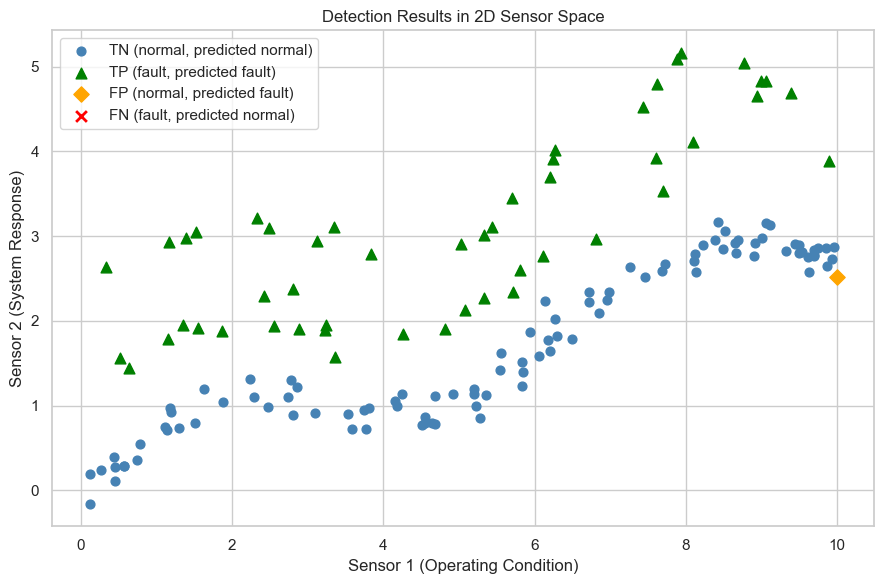
\includegraphics[width=0.78\textwidth]{td7_cell023_img07.png}
  \caption{%
    \textbf{Espacio 2D de sensores con clasificaci\'on de los 150 puntos de test}.
    Cuatro categor\'{\i}as: TP (tri\'angulos verdes) = fallos correctamente detectados;
    TN (c\'{\i}rculos azules) = normales correctamente clasificados; FP (rombos
    naranjas) = falsas alarmas (normales clasificados como fallo); FN (cruces
    rojas) = fallos no detectados. Observar: 1 FP (un punto normal at\'{\i}pico en
    la frontera de la nube normal) y 0 FN (todos los fallos detectados).%
  }
  \label{fig:space2d}
\end{figure}

\caja{La Figura~\ref{fig:space2d} revela d\'onde ocurre el \'unico error de
clasificaci\'on: el FP es un punto normal que por azar se encuentra en el extremo
de la distribuci\'on normal, generando un residuo ligeramente superior al umbral.
No hay ning\'un FN porque los puntos fallados est\'an desplazados lo suficiente
($\geq +1$ unidad) para superar c\'omodamente el umbral de $0.50$.}

\subsubsection{Resultados de clasificaci\'on}

\begin{table}[H]
\centering
\caption{Matriz de confusi\'on --- Detector AAKR ($h=0{,}5$, $\tau \approx 0{,}50$)}
\label{tab:confusion}
\renewcommand{\arraystretch}{1.6}
\setlength{\tabcolsep}{12pt}
\begin{tabular}{l|cc|c}
\toprule
\multirow{2}{*}{\textbf{Real $\backslash$ Predicci\'on}}
  & \textbf{Pred.\ NORMAL}
  & \textbf{Pred.\ FALLO}
  & \textbf{Total} \\
\midrule
\textbf{Real NORMAL}
  & \cellcolor{verdeOK!20}99
  & \cellcolor{rojoFail!20}1
  & 100 \\
\textbf{Real FALLO}
  & \cellcolor{rojoFail!20}0
  & \cellcolor{verdeOK!20}50
  & 50  \\
\midrule
\textbf{Total predicho} & 99 & 51 & 150 \\
\bottomrule
\end{tabular}
\end{table}

\begin{table}[H]
\centering
\caption{M\'etricas de evaluaci\'on del detector}
\label{tab:metrics}
\renewcommand{\arraystretch}{1.45}
\begin{tabular}{>{\bfseries}lcc}
\toprule
\rowcolor{azulTDS!15}
M\'etrica & Valor & F\'ormula \\
\midrule
Accuracy   & 0{,}9933 & $(TP + TN)\;/\;N$ \\
\rowcolor{grisClaro}
Precision  & 0{,}9804 & $TP\;/\;(TP + FP)$ \\
Recall     & 1{,}0000 & $TP\;/\;(TP + FN)$ \\
\rowcolor{grisClaro}
F1 Score   & 0{,}9901 & $2\cdot\text{Precision}\cdot\text{Recall}\;/\;(\text{Precision}+\text{Recall})$ \\
\midrule
Falsos positivos (FP) & 1 & Normal clasificado como fallo \\
\rowcolor{grisClaro}
Falsos negativos (FN) & 0 & Fallo no detectado \\
\bottomrule
\end{tabular}
\end{table}

\subsubsection{An\'alisis de los resultados}

\paragraph{Separaci\'on de distribuciones.}
Los residuos de los datos normales se concentran por debajo de $\approx 0{,}3$
(reconstrucci\'on precisa), mientras que los residuos de los datos fallados se
sit\'uan entre $0{,}8$ y $2{,}2$ (proporcionales al desplazamiento $\Delta$). Las
dos distribuciones tienen escas\'{\i}simo solapamiento, lo que hace que la tarea de
clasificaci\'on sea pr\'acticamente perfecta con un umbral simple.

\paragraph{1 falso positivo, 0 falsos negativos.}
El \'unico error es un punto normal que, por azar, presenta una combinaci\'on de
ruido que lo aleja lo suficiente de la memoria para superar $\tau \approx 0{,}50$.
La probabilidad te\'orica de este evento bajo la regla de los 3 sigmas es
$\approx 0{,}3\,\%$, consistente con 1~FP en 100 puntos normales.

Los 0 falsos negativos son especialmente importantes en el mantenimiento
industrial: un \textbf{fallo no detectado (FN)} puede conducir a una aver\'{\i}a
grave, parada no planificada o accidente. Un \textbf{falso positivo (FP)} solo
desencadena una inspecci\'on innecesaria, con un coste mucho menor.

\paragraph{Compromiso precisi\'on--exhaustividad.}
La elecci\'on del umbral $\tau$ determina directamente el punto de operaci\'on
en la curva ROC. La regla de los 3 sigmas es conservadora (umbral alto): garantiza
pocos FP, pero podr\'{\i}a dejar escapar fallos m\'as sutiles ($\Delta < 0{,}5$).
Para detectarlos, habr\'{\i}a que reducir $\tau$, aceptando m\'as FP a cambio de
mayor exhaustividad (Recall).

% =============================================================
\section{Discusi\'on Comparativa}
% =============================================================

\subsection{AAKR frente a otros m\'etodos de detecci\'on de anomal\'{\i}as}

\begin{table}[H]
\centering
\caption{Comparativa de AAKR con m\'etodos alternativos}
\label{tab:comparison}
\renewcommand{\arraystretch}{1.45}
\begin{tabularx}{\linewidth}{>{\bfseries}p{3cm}
                              >{\centering}X
                              >{\centering}X
                              >{\centering\arraybackslash}X}
\toprule
\rowcolor{azulTDS!15}
M\'etodo & Requiere datos de fallo & Escalabilidad & Interpretabilidad \\
\midrule
AAKR & No & Baja & Alta \\
\rowcolor{grisClaro}
PCA / DPCA & No & Alta & Media \\
Isolation Forest & No & Alta & Baja \\
\rowcolor{grisClaro}
Autoencoder & No & Alta & Baja \\
SVM (One-Class) & No & Media & Media \\
\rowcolor{grisClaro}
Random Forest & S\'{\i} & Alta & Media \\
LSTM / TCN & S\'{\i} (ideal) & Alta & Baja \\
\bottomrule
\end{tabularx}
\end{table}

\subsection{Ventajas de AAKR}

\begin{enumerate}[leftmargin=2em]
  \item \textbf{Aprendizaje no supervisado de anomal\'{\i}as.} Solo requiere datos
        normales, que son abundantes en sistemas industriales. Los datos de fallo
        son escasos, costosos de obtener y dif\'{\i}ciles de etiquetar.

  \item \textbf{Sin fase de entrenamiento.} La memoria se construye en tiempo
        lineal $\mathcal{O}(n)$ y puede actualizarse en tiempo real simplemente
        a\~nadiendo o eliminando observaciones.

  \item \textbf{Modela correlaciones entre sensores.} Al operar sobre vectores
        $\mathbf{x} \in \mathbb{R}^d$, AAKR captura la relaci\'on entre todos los
        sensores simult\'aneamente. Un fallo que afecta solo a un sensor rompe esta
        correlaci\'on y genera un residuo grande.

  \item \textbf{Interpretabilidad del residuo.} El residuo $r_q$ tiene unidades
        f\'{\i}sicas (las mismas que los sensores) y puede descomponerse por componentes
        para identificar \emph{qu\'e} sensor est\'a fallando y \emph{cu\'anto} se ha
        desviado.

  \item \textbf{Umbral adaptable.} La regla de los 3 sigmas proporciona un punto
        de partida robusto, pero el umbral puede ajustarse seg\'un la tolerancia al
        riesgo de la aplicaci\'on.
\end{enumerate}

\subsection{Limitaciones de AAKR}

\begin{enumerate}[leftmargin=2em]
  \item \textbf{Escalabilidad.} El coste de predicci\'on es $\mathcal{O}(nm)$ para
        $m$ consultas y $n$ puntos de memoria. Para $n$ grande (millones de
        observaciones), esto puede ser prohibitivo. Soluciones: submuestreo de la
        memoria, estructuras $k$-d tree, o aproximaciones de kernel.

  \item \textbf{Sensibilidad a $h$.} La elecci\'on del ancho de banda requiere
        validaci\'on cruzada o conocimiento experto. Un $h$ mal calibrado genera
        muchos FP ($h$ peque\~no) o no detecta fallos peque\~nos ($h$ grande).

  \item \textbf{Datos normales heterog\'eneos.} Si el comportamiento normal var\'{\i}a
        significativamente (e.g., distintos reg\'{\i}menes de operaci\'on), AAKR puede
        generar residuos grandes en zonas poco pobladas de la memoria, incluso para
        observaciones normales.

  \item \textbf{Maldici\'on de la dimensionalidad.} La distancia euclidiana pierde
        significado cuando $d$ es grande. En espacios de alta dimensi\'on conviene
        normalizar las variables o aplicar reducci\'on de dimensionalidad previa.

  \item \textbf{Fallos correlacionados sutiles.} Si el fallo desplaza m\'ultiples
        sensores de forma consistente con la variedad normal, el residuo puede ser
        peque\~no y el fallo no se detecta.
\end{enumerate}

\subsection{Conexi\'on con el estimador de Nadaraya-Watson}

AAKR pertenece a la familia de los \emph{estimadores de Nadaraya-Watson}, que son
la base de la regresi\'on no param\'etrica por kernel. Matem\'aticamente, la
predicci\'on de AAKR coincide exactamente con este estimador cuando se usa un
kernel gaussiano isotr\'opico. Por tanto, AAKR hereda las propiedades te\'oricas
bien establecidas de ese estimador:
\begin{itemize}[leftmargin=2em]
  \item \emph{Consistencia}: convergencia en media cuadr\'atica a la funci\'on de
        regresi\'on verdadera cuando $n \to \infty$, $h \to 0$ y $nh \to \infty$.
  \item \emph{Tasa \'optima}: $\mathcal{O}(n^{-4/(d+4)})$ bajo condiciones de
        suavidad est\'andar.
\end{itemize}

\subsection{Aplicaciones industriales reales}

AAKR y sus variantes se han desplegado con \'exito en los siguientes dominios
industriales:

\begin{itemize}[leftmargin=2em]
  \item \textbf{Energ\'{\i}a nuclear}: monitorizaci\'on de temperaturas y presiones en
        el circuito primario de reactores (aplicaci\'on original de Mott et al.).
  \item \textbf{Turbinas e\'olicas}: detecci\'on de fallos en cojinetes, generadores
        y palas a partir de se\~nales de vibraci\'on y temperatura.
  \item \textbf{Aviaci\'on}: monitorizaci\'on de salud de motores de avi\'on (Engine
        Health Management), donde los fallos deben detectarse con m\'{\i}nimos FN.
  \item \textbf{Ferrocarril}: detecci\'on de anomal\'{\i}as en sistemas de frenado y
        rodadura.
  \item \textbf{Procesos qu\'{\i}micos}: monitorizaci\'on de reactores, columnas de
        destilaci\'on y compresores.
\end{itemize}

En todos estos casos, la propiedad clave es la misma: el comportamiento normal est\'a
bien caracterizado (muchas horas de operaci\'on sin fallos) y los datos de fallo son
escasos o no disponibles en el momento del dise\~no del sistema.

% =============================================================
\section{Conclusiones}
% =============================================================

Este TD ha demostrado que AAKR es un algoritmo simple, elegante y efectivo para
la detecci\'on de fallos en sensores industriales. Las principales conclusiones son:

\begin{enumerate}[leftmargin=2em, label=\textbf{\arabic*.}]

  \item \textbf{Implementaci\'on directa y vectorizable.} Los tres pasos del
        algoritmo (distancias, kernel, media ponderada) se implementan en menos
        de 10 l\'{\i}neas de \texttt{NumPy} con vectorizaci\'on completa. La extensi\'on
        al caso multidimensional no requiere cambios conceptuales: basta sustituir
        las distancias escalares por \texttt{cdist} euclidiana.

  \item \textbf{Calidad de predicci\'on competitiva.} Con $h$ bien elegido, AAKR
        alcanza un MSE del orden del nivel de ruido ($\approx 0{,}02$ para
        $\sigma = 0{,}15$), recuperando fielmente la funci\'on $\sin(x)$ subyacente
        sin especificar ninguna forma funcional \emph{a priori}.

  \item \textbf{El ancho de banda $h$ es el \'unico hiperpar\'ametro cr\'{\i}tico.}
        La curva MSE en funci\'on de $h$ tiene forma de U: valores peque\~nos
        producen sobreajuste (solo el vecino m\'as cercano) y valores grandes
        producen infraajuste (media global). El \'optimo en el dataset 1-D
        analizado es $h \approx 0{,}3$, identificado por barrido sistem\'atico.

  \item \textbf{Visualizaci\'on de pesos como herramienta de diagn\'ostico.}
        La distribuci\'on de pesos $\tilde{w}_i$ para un punto de consulta
        dado revela directamente si el modelo est\'a en r\'egimen de overfitting
        (spike), underfitting (uniforme) o ajuste \'optimo (campana estrecha).

  \item \textbf{Detecci\'on de fallos casi perfecta.} En el escenario bidimensional
        con fallos de drift ($+1{,}0$) y bias ($+2{,}0$), AAKR alcanza:
        Accuracy = 99{,}33\,\%, Recall = 100\,\% (0 fallos no detectados) y
        F1 = 99{,}01\,\%. El \'unico error es 1 falso positivo, irrelevante en
        mantenimiento industrial.

  \item \textbf{El mecanismo de detecci\'on es intuitivo y f\'{\i}sicamente
        interpretable.} La memoria normal permite reconstruir con alta precisi\'on
        observaciones normales (residuo peque\~no), pero no puede reconstruir
        observaciones falladas porque est\'an fuera de la variedad normal (residuo
        grande). La regla de los 3 sigmas proporciona un umbral robusto e
        interpretable con tasa de falsas alarmas te\'orica del 0{,}3\,\%.

  \item \textbf{Aplicabilidad y limitaciones industriales.} AAKR es id\'oneo para
        sistemas con comportamiento normal bien caracterizado y datos de fallo
        escasos o no disponibles. Su principal limitaci\'on es la escalabilidad:
        para memorias de millones de observaciones se requieren aproximaciones
        (submuestreo, $k$-d trees). En sistemas con alta dimensionalidad o
        m\'ultiples reg\'{\i}menes de operaci\'on, se recomienda complementarlo con
        reducci\'on de dimensionalidad o agrupamiento previo.

\end{enumerate}

\vspace{1cm}
\noindent\rule{\linewidth}{0.8pt}
\begin{center}
  \small\itshape
  Documento elaborado para el curso de Machine Learning Industrial.\\
  \'Oscar Mart\'{\i}nez Zamora --- Junio 2026.
\end{center}

\end{document}
